%%%%%%%%%%%%%%%%%%%%%%%%%%%%%%%%%%%%%%%%%
% Template LaTeX Template Version 1.0 (December 8 2014)
%
% This template has been downloaded from: http://www.LaTeXTemplates.com
%
% Original author: Brandon Fryslie With extensive modifications by: Vel
% (vel@latextemplates.com)
%
% License: CC BY-NC-SA 3.0 (http://creativecommons.org/licenses/by-nc-sa/3.0/)
%
% Authors: Sabbir Ahmed, Jeffrey Osazuwa, Howard To, Brian Weber
% 
%%%%%%%%%%%%%%%%%%%%%%%%%%%%%%%%%%%%%%%%%

\documentclass[12pt]{extarticle}
%%%%%%%%%%%%%%%%%%%%%%%%%%%%%%%%%%%%%%%%%
% Structure
% Structural Definitions File
% Version 1.0 (December 8 2014)
%
% Created by:
% Vel (vel@latextemplates.com)
% 
% This file has been downloaded from:
% http://www.LaTeXTemplates.com
%
% License:
% CC BY-NC-SA 3.0 (http://creativecommons.org/licenses/by-nc-sa/3.0/)
%
%%%%%%%%%%%%%%%%%%%%%%%%%%%%%%%%%%%%%%%%%

\usepackage{geometry} % Required to modify the page layout

\usepackage{amsmath}
\usepackage{amssymb}

\usepackage[utf8]{inputenc} % Required for including letters with accents
\usepackage[T1]{fontenc} % Use 8-bit encoding that has 256 glyphs

\usepackage{avant} % Use the Avantgarde font for headings
\usepackage{setspace}

\setlength{\parindent}{0mm} % Don't indent paragraphs
\setlength{\parskip}{2.5mm} % Whitespace between paragraphs

\setlength{\textwidth}{16cm} % Width of the text on the page
\setlength{\textheight}{23cm} % Height of the text on the page
\setlength{\oddsidemargin}{0cm} % Width of the margin - negative to move text left, positive to move it right
\setlength{\topmargin}{-1.25cm} % Reduce the top margin

\renewcommand\familydefault{\sfdefault}  % default font for entire document
 % specifies the document layout and style

% names
\newcommand{\team}{Galois Field Arithmetic Unit}
\newcommand{\Sabbir}{Sabbir Ahmed}
\newcommand{\Jeffrey}{Jeffrey Osazuwa}
\newcommand{\Howard}{Howard To}
\newcommand{\Brian}{Brian Weber}

% document info command
\newcommand{\documentinfo}[5]{
    \begin{centering}
        \parbox{2in}{
        \begin{spacing}{1}
            \begin{flushleft}
                \begin{tabular}{l l} #1 \\ #2 \\ #3 \\ #4 \\ #5 \\
                \end{tabular}\\
                \rule{\textwidth}{1pt}
            \end{flushleft}
        \end{spacing} }
    \end{centering} }

\graphicspath{ {diagrams/} }
\renewcommand{\baselinestretch}{1.5}
\setenumerate[1]{label=\thesubsection.\arabic*., leftmargin=3.5em}
\setenumerate[2]{label*=\arabic*.}

\begin{document}

    \documentinfo {\textbf{MEMO NUMBER:} GFAU SRS} {\textbf{DATE:} \today}
    {\textbf{TO: } EFC LaBerge} {\textbf{FROM: }\Sabbir, \Jeffrey, \Howard,
    \Brian} {\textbf{SUBJECT: } System Requirement Specifications}
    \vspace{-0.1in}

    \section{Introduction} A Galois Field is a field with a finite number of
    elements. The nomenclature $GF(q)$ is used to indicate a Galois Field with
    $q$ elements. In $GF(q)$, the parameter $q$ must be a power of a prime. For
    each prime power there exists exactly one finite field. The binary field
    $GF(2)$ is the most frequently used Galois field \cite{wolfdef}.

    The \team~will handle irreducible polynomials in $GF(2^n)$, where $2 \leq
    n \leq 16$. The arithmetic logic unit (ALU) will generate all the terms in
    the field of the polynomial, and allow the user to view and apply the
    following Galois operations: addition, subtraction, multiplication,
    division and logarithm.

        \subsection{Document Overview} This document serves as the System
        Requirements Specification for the Galois Field Arithmetic Unit. The
        description and requirements of the project are embodied in this
        document.

        The Specification is divided into separate segments pertaining to
        individual components and requirements on different levels. Figures and
        tables are attached where necessary to assist in demonstrating
        concepts.

        \subsection{Mission Scenario} Galois Fields have various applications
        in error detection and correction (EDAC). Specifically, cyclic
        redundancy checks (CRC) is an EDAC that employ $GF(2)$ \cite{crc}.
        EDAC has many expensive calculations that are difficult for low power
        and inexpensive microcontrollers to handle. The GFAU will make Galois
        Field computations more accessible to such low powered devices.
        \newpage

        \section{System Overview} The GFAU prototype will be composed of
        discrete modules residing in a single programmable board. Individual
        modules will be programmed to solely complete an assigned task.
        Although modules are assigned individual tasks, they should not have
        exclusive components for its functionality.

        \subsection{System Boundary Diagram} Figure \ref{fig:system_boundary} provides the System Boundary Diagram of the GFAU.

        \begin{figure}[ht]
            \begin{center}
                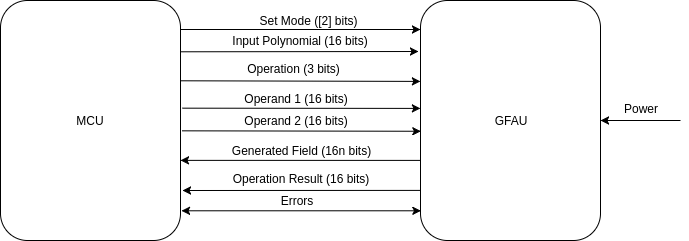
\includegraphics[width=1\textwidth]{system_boundary.png}
                \caption{System Boundary Diagram of the \team~, where $n$ is
                the Number of Terms} \label{fig:system_boundary}
            \end{center}
        \end{figure}

        The user I/O interface are handled by the external device which are
        transferred via busses. The user inputs consist of the mode bit, the
        input generating polynomial and the binary operation(s) along with
        their corresponding operands. The external device transfers the data to
        the unit to perform the desired operations. The GFAU will return the
        outputs and any errors detected back to the external device.
        \newpage

        \subsection{Functional Flow Diagram} Figure \ref{fig:functional_flow}
        provides the functional flow of the GFAU.

        \begin{figure}[ht]
            \begin{center}
                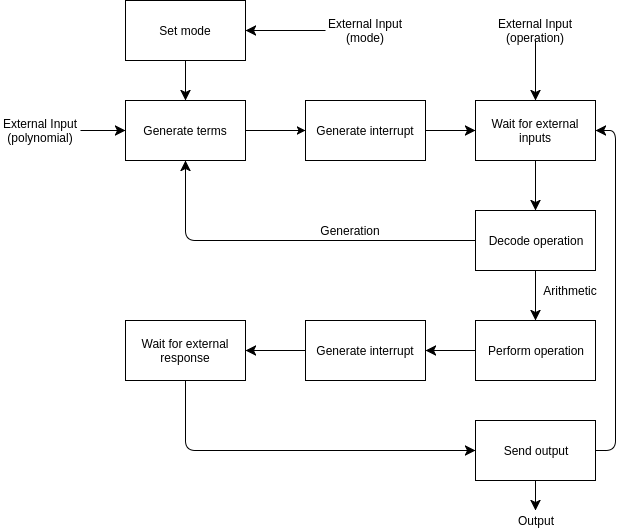
\includegraphics[width=1\textwidth]{functional_flow.png}
                \caption{Functional Flow Diagram of the \team~}
                \label{fig:functional_flow}
            \end{center}
        \end{figure}

        The diagram provides a high-level overview of the sequence of processes
        that take place in the unit. In total, the unit waits for an input from
        the user in three separate instances. The order of the inputs are
        essential for the unit to proceed as desired. The \textbf{mode} input
        sets the width of the data bus in the GFAU. The \textbf{polynomial}
        input consist of the generating polynomial to generate its terms in the
        Galois field. The \textbf{operation} input consists of the two operands
        along with the desired binary operation.
        \newpage

        \subsection{Data Flow Diagram} Figure \ref{fig:data_flow} provides the
        data flow diagram of the GFAU.

        \begin{figure}[ht]
            \begin{center}
                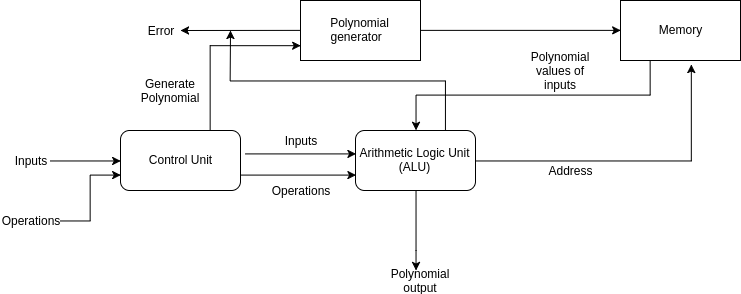
\includegraphics[width=1\textwidth]{data_flow.png}
                \caption{Data Flow Diagram of the \team~} \label{fig:data_flow}
            \end{center}
        \end{figure}

        The diagram provides a lower-level view of the system emphasizing the
        individual components and their role in converting the input data to
        the desired output. The \textbf{Error} lines are used by multiple
        components to send interrupt signals to the user when required.
        \newpage

    \section{Requirements}

        \subsection{Functional Requirements} The GFAU shall perform the
        functions outlined below.

        \begin{enumerate}

            \item The GFAU shall generate terms from input irreducible
            polynomials of degrees 2 to 8.

            \item The GFAU shall handle operations on terms from $GF(2)$ to
            $GF(8)$.

            \item The GFAU should generate terms from input irreducible
            polynomials of degrees 2 to 16.

            \item The GFAU should handle operations on terms from $GF(2)$ to
            $GF(16)$.

            \item The GFAU shall perform addition, subtraction, multiplication,
            division, and logarithm operations in the Galois Field.

            \item The GFAU shall handle inputs given in their element or
            polynomial from depending on the opcode provided from the external
            device.

            \item The GFAU shall be able to generate outputs in their element
            or polynomial depending on the opcode from the external device.


        \end{enumerate}

        \subsection{Cost and Package Constraints} This section outlines all
        design constraints imposed by the customer, from which the remainder of
        the requirements are derived.

        \begin{enumerate}

            \item The total cost of the prototype shall not exceed \$400.

            \item The total area of prototype printed circuit board (PCB) shall
            not exceed 24 inches square.

            \item The cost at mass production shall not exceed \$1 per chip.

            \item The package of the final product shall not exceed 64 pins and
            should use fewer than 64 pins.

        \end{enumerate}

        \subsection{Hardware Requirements} The GFAU shall prioritize hardware
        portability, as it provides flexibility in the ranges of its
        specifications. The hardware specifications shall include reasonably
        bounded ranges.

        \begin{enumerate}

            \item The GFAU shall be functional at a variety of clock speeds at
            a minimum range of [4 MHz - 100 MHz].

            \item The GFAU shall not exceed a thermal design power (TDP) of [1]
            W in a final implementation.

            \item The GFAU shall operate normally at a temperature range of
            -40$^{\circ}$C to \textasciitilde 85$^{\circ}$C.

            \item The input voltage for the unit shall be [5] V.

        \end{enumerate}

        \subsection{Software and Testing Requirements} Software testing through
        extensive simulations in hardware description language (HDL) shall be
        incorporated into the requirements of the GFAU. Simulations allow for
        convenient debugging and minimizes the risks of unintended behavior in
        the prototype. Before purchasing hardware, the HDL code shall pass the
        following required tests.

        \begin{enumerate}

            \item All HDL code shall be synthesizable.

            \item The simulations shall prove the HDL code functions, as
            intended, with [99\%] certainty.

            \item During verification, values (such as gate delays) shall be
            parametrized to readily match the specifications of candidate
            hardware.

        \end{enumerate}

        \subsection{Signal Testing and Requirements} To ensure that all
        communication occurs accurately between the external device and the
        GFAU, all output signals shall not exceed rise and fall times of [1
        ns]. All signals shall incorporate an oscilloscope to measure their
        timings. A digital logic analyzer shall be used to verify the output
        signals.

        \subsection{Communication Requirements} The GFAU shall be able to
        communicate with a wide variety of external devices with commonly used
        communication methods outlined below.

        \begin{enumerate}

            \item The GFAU shall provide the external device the option to
            select between a 8, 16, [or 32] bit data-bus.

            \item The GFAU shall set a ready pin after the completion of the
            given operation.

            \item The GFAU shall allow the external device to use polling or
            interrupts to monitor the ready pin to pull the data from the bus.

            \item The GFAU shall push relatively small blocks of data over a
            bus to the external device using a common or easy-to-implement
            protocol on one clock.

        \end{enumerate}

        \subsubsection*{3.6 (A) \ \ Error Codes} Error signals shall be sent to the
        external device in the following cases.

        \begin{enumerate}[resume]

            \item The GFAU shall produce an error if its input polynomial
            is reducible.
            
            \item The GFAU shall produce an error if an operand exceeds the
            bounds Galois Field generated by the input polynomial.
            
            \item The GFAU shall produce an error if an operand is
            attempted to be divided by 0 (zero).
            
            \item The GFAU shall produce an error if it does not receive
            all the inputs from the external device.

        \end{enumerate}

        \begin{thebibliography}{2}
            \bibitem{wolfdef}
            Wolfram Math World, "Finite Field." \textit{Wolfram Math World},
            2017. [Online document]. Availble:
                  http://mathworld.wolfram.com/FiniteField.html. [Accessed:
                  Nov. 21, 2017].

            \bibitem{crc} 
            N. Matloff , "Cyclic Redundancy Checking." \textit{University of
               California at Davis}, 2001. [Online]. Availble: http://heather.c
               s.ucdavis.edu/~matloff/Networks/CRC/Old/ErrChkCorr.html.
               [Accessed: Nov. 21, 2017].
        \end{thebibliography}


\end{document}
